% Background, ueberarbeitete Fassung. Aufbau: 1 PES, 2 Electronic structure,
% 3 NEB, 4 MLIPs, 5 Datasets. Abschnitte, die der Delta-Chat entscheidet,
% sind mit "% (Delta)" markiert und stehen zunaechst wie im Entwurf.
% Quelle des Entwurfs: docs/chapter_background.tex (Kopie aus der Thesis).
% Referenzen: docs/background_refs.bib.
%
% Stand: Abschnitt 1 geschrieben (2026-09-07). 2 bis 5 folgen.

\chapter{Background}
\label{ch:background}

% =====================================================================
\section{Potential Energy Surfaces}
\label{sec:background-pes}

\subsection{The Born--Oppenheimer Surface}
\label{sec:background-bo}

Nuclei are thousands of times heavier than electrons. On the timescale of
nuclear motion the electrons adjust instantly, so the electronic problem can
be solved with the nuclei held fixed at positions $\mathbf{R}$,
%
\begin{equation}
  \hat{H}_\text{el}(\mathbf{R})\, \psi_k(\mathbf{r};\mathbf{R})
  = E_k(\mathbf{R})\, \psi_k(\mathbf{r};\mathbf{R}),
  \qquad E_0 \le E_1 \le \dots
  \label{eq:electronic-schrodinger}
\end{equation}
%
The lowest eigenvalue $E_0(\mathbf{R})$, computed for every nuclear
arrangement, is the potential energy surface (PES). The nuclei move on it and
feel the force $-\nabla E_0(\mathbf{R})$. The approximation holds when the
ground state is well separated from the excited states.

\subsection{Stationary Points}
\label{sec:background-stationary}

The chemistry of a surface lies in its stationary points, where the gradient
$\mathbf{g} = \nabla_\mathbf{R} E$ vanishes. The eigenvalues of the Hessian
$\mathbf{H}_{ij} = \partial^2 E / \partial R_i \partial R_j$ tell them apart:

\begin{itemize}
  \item \textbf{Local minima} ($\mathbf{H}$ positive definite) are stable or
    metastable structures --- the reactants and products of a reaction.
  \item \textbf{First-order saddle points} (exactly one negative eigenvalue)
    are \textbf{transition states} (TS): the highest point on the
    lowest-energy path between two minima. The eigenvector of the negative
    eigenvalue is the reaction coordinate at the TS.
\end{itemize}

The energy difference between transition state and reactant is the barrier
$\Delta E^\ddagger$. Transition state theory relates it to the rate constant
by $k \propto \exp(-\Delta E^\ddagger / k_\text{B} T)$~\cite{eyring1935}, so
an error in the barrier enters the rate exponentially. An error of
1~kcal/mol (43~meV) changes the rate at room temperature by a factor of
five; this value is called chemical accuracy.

\subsection{Geometry and Energy}
\label{sec:geom-energy}

A barrier calculation has two parts: the geometry of the transition state,
and the energy of the surface at that geometry relative to the reactant. The
two can be computed with different methods. A geometry optimised with one
method can be used for an energy calculation with another, a single-point
calculation. A reference calculation therefore has a geometry level and an
energy level. Common practice lets the geometry level be the lower one,
because structures depend less on functional and basis set than
energies~\cite{bursch2022}.

% =====================================================================
\section{Electronic Structure Methods}
\label{sec:background-electronic}

An electronic structure method solves Eq.~\eqref{eq:electronic-schrodinger}
approximately by restricting the form of the wavefunction. It returns the
lowest energy within that form and its gradient. If the true ground state
lies outside the form, the method returns a higher state without indication.

\subsection{Single-Reference and Multireference Systems}
\label{sec:sr-vs-mr}

Electrons occupy orbitals, each holding at most two electrons of opposite
spin. One assignment of all electrons to orbitals is a configuration, written
as a Slater determinant $\Phi_I$. An electronic state is a weighted sum of
determinants,
%
\begin{equation}
  \Psi = \sum_I c_I \, \Phi_I ,
  \qquad \sum_I |c_I|^2 = 1 .
  \label{eq:ci-expansion}
\end{equation}
%
At most geometries one determinant carries nearly all the weight; this is the
single-reference case, and Hartree--Fock, Kohn--Sham DFT and coupled cluster
are built for it. Where a bond is half broken, two configurations carry
comparable weight: the electron pair shares one orbital, or one electron sits
on each fragment. This is the multireference case. It can be treated with
several determinants (Section~\ref{sec:background-mr}), or with one
determinant in which the two electrons may occupy different orbitals
(Section~\ref{sec:background-spin}). The second is the broken-symmetry
approach.

% ─────────────────────────────────────────────────────────
\subsection{Density Functional Theory}
\label{sec:background-dft}

Kohn--Sham DFT builds the electron density from one determinant of orbitals
and puts everything beyond that determinant into the exchange--correlation
functional. The orbitals are found by the self-consistent field (SCF)
iteration: orbitals give a density, the density gives a potential, the
potential gives new orbitals, until nothing changes. The result is a
stationary point of the energy in the space of orbitals. It is the one the
starting guess leads to, and not necessarily the lowest. The functional and
the basis set together define the level of theory.

% (Delta) Die folgenden Abschnitte -- Many-body problem, Kohn--Sham und das
% XC-Funktional, Jacobs Ladder, Hybrid/Range-Separation/Dispersion, die zwei
% Funktionale, Basissaetze -- stehen wortgleich wie im Entwurf. Laenge,
% Grafiken und Kuerzungen entscheidet der Delta-Chat. Fuer das OMol25-Kapitel
% wird daraus nur gebraucht: (a) der SCF-Absatz "Two properties of this
% procedure matter later" im Kohn--Sham-Abschnitt, (b) dass Funktional plus
% Basis das Level bilden.
\subsubsection{The Many-Body Problem and the Key Insight of DFT}

Solving the electronic Schrödinger equation exactly for a molecule with $N_e$
electrons requires knowing the full many-body wavefunction
$\Psi(\mathbf{r}_1, \ldots, \mathbf{r}_{N_e})$ --- a function of $3N_e$ spatial
coordinates. For even a modest molecule of 20 electrons this is a function in 60
dimensions, and the computational cost of exact diagonalisation grows
exponentially with $N_e$. No practical calculation is possible beyond a handful
of electrons.

Density functional theory (DFT) offers a radical simplification. The
Hohenberg--Kohn theorems (1964) prove that the ground-state energy of an
electronic system is a unique functional of the electron density
$\rho(\mathbf{r})$ alone --- a function of just three spatial coordinates,
regardless of the number of electrons. Knowing $\rho(\mathbf{r})$ is in principle
sufficient to determine everything about the ground state. The many-body problem
in $3N_e$ dimensions collapses to a problem in 3 dimensions.

\subsubsection{The Kohn--Sham Approach and the Exchange--Correlation Functional}

In practice, the exact density functional is unknown. Kohn and Sham (1965)
reformulated the problem by introducing a fictitious system of \emph{non-interacting}
electrons moving in an effective potential chosen so that their density exactly
matches the true interacting density. The non-interacting electrons occupy
single-particle orbitals $\phi_i(\mathbf{r})$ (the Kohn--Sham orbitals), and
the total energy is:

\begin{equation}
  E[\rho] = T_s[\rho] + E_\text{ext}[\rho] + E_\text{Hartree}[\rho]
            + E_\text{XC}[\rho],
\end{equation}

where $T_s$ is the kinetic energy of the non-interacting electrons, $E_\text{ext}$
is the electron--nuclear attraction, $E_\text{Hartree}$ is the classical
electron--electron repulsion, and $E_\text{XC}$ --- the
\textbf{exchange--correlation (XC) functional} --- captures everything else:
quantum mechanical exchange, electron correlation, and the correction to the
kinetic energy from the real interacting system. The first three terms are computed
exactly. Only $E_\text{XC}$ must be approximated.

The Kohn--Sham equations are solved iteratively, because the effective potential
in which the orbitals move depends on the density that those same orbitals
produce. Starting from an initial guess for the orbitals, one constructs the
effective potential, solves for a new set of orbitals, forms the new density, and
repeats until the density no longer changes --- the \textbf{self-consistent
field} (SCF) procedure. The converged result is a stationary point of the energy
with respect to variation of the orbitals. Two properties of this procedure
matter later: the outcome can depend on the initial guess, since the iteration
converges to whichever stationary point it is drawn towards; and a converged
solution is stationary but not necessarily the lowest one, a distinction taken up
in Section~\ref{sec:background-stability}.

The exchange--correlation functional is the central approximation in DFT, and
the accuracy of any DFT calculation depends almost entirely on the quality of
this approximation. Decades of development have produced a hierarchy of increasingly
sophisticated approximations, commonly organised on \textbf{Jacob's ladder}
(Figure~\ref{fig:jacobs-ladder}), ascending from crude local approximations to
highly accurate nonlocal ones.

\begin{figure}[h]
\centering
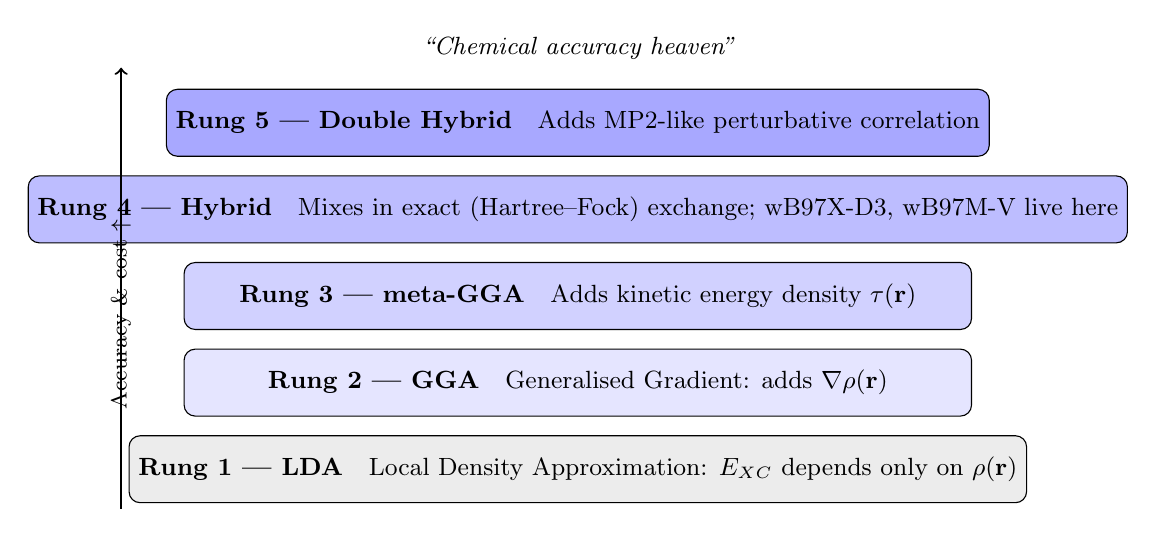
\begin{tikzpicture}[
  rung/.style={draw, rounded corners=4pt, fill=#1, minimum width=10cm,
               minimum height=0.85cm, align=center, font=\small},
  lbl/.style={font=\footnotesize, align=left, text width=4.5cm},
]
% Rungs bottom to top
\node[rung=gray!15]    (r1) at (0,0.00) {\textbf{Rung 1 — LDA}\quad
  Local Density Approximation: $E_\text{XC}$ depends only on $\rho(\mathbf{r})$};
\node[rung=blue!10]    (r2) at (0,1.10) {\textbf{Rung 2 — GGA}\quad
  Generalised Gradient: adds $\nabla\rho(\mathbf{r})$};
\node[rung=blue!18]    (r3) at (0,2.20) {\textbf{Rung 3 — meta-GGA}\quad
  Adds kinetic energy density $\tau(\mathbf{r})$};
\node[rung=blue!26]    (r4) at (0,3.30) {\textbf{Rung 4 — Hybrid}\quad
  Mixes in exact (Hartree--Fock) exchange; \mbox{wB97X-D3}, \mbox{wB97M-V} live here};
\node[rung=blue!34]    (r5) at (0,4.40) {\textbf{Rung 5 — Double Hybrid}\quad
  Adds MP2-like perturbative correlation};

% Heaven label
\node[font=\small\itshape] at (0, 5.35) {``Chemical accuracy heaven''};

% Arrow on the left
\draw[->, thick] (-5.8,-0.5) -- (-5.8,5.1)
  node[midway, left, font=\footnotesize, align=center, rotate=90,
       xshift=1cm] {Accuracy \& cost $\uparrow$};

\end{tikzpicture}
\caption{Jacob's ladder of density functional approximations. Each rung adds
more physical ingredients to the exchange--correlation functional, generally
increasing accuracy at the cost of computational expense. Both functionals used
in this thesis sit on Rung~4: \mbox{wB97X-D3} as a hybrid GGA and \mbox{wB97M-V}
as a hybrid meta-GGA.}
\label{fig:jacobs-ladder}
\end{figure}

\subsubsection{Hybrid Functionals and Range Separation}

Rung~4 hybrid functionals improve upon lower rungs by mixing a fraction of
\emph{exact exchange} --- the exchange energy computed from the Kohn--Sham
orbitals as in Hartree--Fock theory --- into the approximate XC functional.
This reduces self-interaction error and generally improves barrier heights, which
are systematically underestimated by GGA and meta-GGA functionals.

\textbf{Range-separated} hybrids go further by splitting the electron--electron
interaction into short-range and long-range components using a partitioning
parameter $\omega$:
%
\begin{equation}
  \frac{1}{r_{12}} = \underbrace{\frac{1-\text{erf}(\omega r_{12})}{r_{12}}}_{\text{short range (DFT)}}
  + \underbrace{\frac{\text{erf}(\omega r_{12})}{r_{12}}}_{\text{long range (HF exchange)}}.
\end{equation}
%
At short range, the DFT exchange approximation is accurate. At long range, exact
exchange is used instead, correctly describing charge-transfer interactions and
improving the asymptotic behaviour of the potential. The $\omega$B97 family of
functionals exploits this splitting.

\textbf{Dispersion corrections} address a further weakness of standard DFT: the
inability to describe van der Waals (London dispersion) interactions, which arise
from correlated fluctuations in electron density and are entirely absent from local
XC approximations. The D3 correction~\cite{grimme2010} adds atom-pairwise damped
$C_6/r^6$ terms to the DFT energy; the VV10 non-local correlation
functional~\cite{vydrov2010} takes a more principled approach by computing
dispersion from a double integral over the electron density. Both approaches
correct the same physics; VV10 is generally more accurate for strongly interacting
pairs.

\subsubsection{The Two Functionals in This Work}

\textbf{\mbox{wB97X-D3/6-31G(d)}}~\cite{lin2013} is a range-separated hybrid
GGA with D3 pairwise dispersion. It was chosen for generating Transition1x due to
its good overall performance and affordable cost. Its main limitations for this
thesis are the small basis set (discussed below) and the absence of kinetic energy
density (a Rung~3 ingredient), which limits its accuracy for barrier heights
relative to meta-GGA functionals.

\textbf{\mbox{wB97M-V/def2-TZVP}}~\cite{mardirossian2016} is a range-separated
hybrid \emph{meta}-GGA with VV10 non-local dispersion. The additional kinetic
energy density ingredient adds a Rung~3 ingredient the other functional lacks, and
VV10 is more physically rigorous than pairwise D3 for dispersion. In the
comprehensive GMTKN55 benchmark~\cite{goerigk2017}, \mbox{wB97M-V} consistently
ranks among the most accurate Rung~4 functionals for thermochemistry, kinetics,
and non-covalent interactions. It is used as the NEB refinement level and the
target level for the delta learning approach in this thesis.

% ─────────────────────────────────────────────────────────
\subsection{Basis Sets}
\label{sec:background-basis}

\subsubsection{Representing Molecular Orbitals}

A Kohn--Sham orbital $\phi_i(\mathbf{r})$ is a function of continuous space.
To make it computable, it must be represented in a finite set of known
functions --- a \textbf{basis set}. The standard approach (LCAO: linear combination
of atomic orbitals) expresses each molecular orbital as a sum over atom-centred
basis functions $\chi_\mu$:

\begin{equation}
  \phi_i(\mathbf{r}) = \sum_\mu c_{\mu i}\, \chi_\mu(\mathbf{r} - \mathbf{R}_A),
\end{equation}

where $\mathbf{R}_A$ is the position of atom $A$ and the coefficients $c_{\mu i}$
are determined variationally. In practice, each basis function $\chi_\mu$ is a
\textbf{contracted Gaussian-type orbital} (GTO): a fixed linear combination of
Gaussian functions $e^{-\alpha_k |\mathbf{r}|^2}$ with different exponents
$\alpha_k$, centred on the atom. Gaussians are used because integrals of products
of Gaussians can be evaluated analytically, making the construction of the Kohn--Sham
matrix efficient.

The key parameters of a basis set are its \textbf{size} (how many basis functions
per atom) and its \textbf{composition} (which angular momentum types are included).
Larger basis sets represent the orbital more accurately but increase computational
cost as $\mathcal{O}(N_\text{basis}^4)$ for DFT. Figure~\ref{fig:basis-sets}
illustrates the two basis sets used in this thesis.

\begin{figure}[h]
\centering
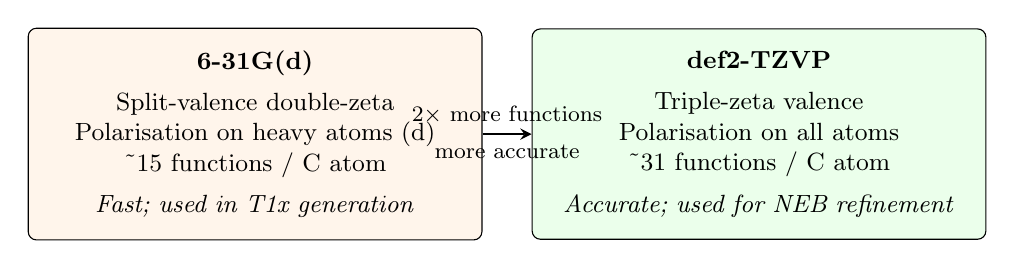
\begin{tikzpicture}[
  box/.style={draw, rounded corners=3pt, align=center, minimum height=2.2cm,
              text width=5.2cm, font=\small, inner sep=8pt},
  arr/.style={->, thick, >=stealth},
]

\node[box, fill=orange!8] (small) at (-3.2,0) {
  \textbf{6-31G(d)} \\[4pt]
  Split-valence double-zeta \\
  Polarisation on heavy atoms (d) \\
  \textasciitilde 15 functions / C atom \\[4pt]
  \textit{Fast; used in T1x generation}
};

\node[box, fill=green!8] (large) at (3.2,0) {
  \textbf{def2-TZVP} \\[4pt]
  Triple-zeta valence \\
  Polarisation on all atoms \\
  \textasciitilde 31 functions / C atom \\[4pt]
  \textit{Accurate; used for NEB refinement}
};

\draw[arr] (small.east) -- (large.west)
  node[midway, above, font=\footnotesize] {$2\times$ more functions}
  node[midway, below, font=\footnotesize] {more accurate};

\end{tikzpicture}
\caption{The two basis sets used in this thesis. A larger, more complete basis
set reduces the \emph{basis set incompleteness error} at increased computational
cost.}
\label{fig:basis-sets}
\end{figure}


\subsubsection{Reading a Method Specification: wB97X-D3/6-31G(d)}

A method specification like \mbox{wB97X-D3/6-31G(d)} encodes two independent
choices separated by a slash: the \textbf{functional} (wB97X-D3) and the
\textbf{basis set} (6-31G(d)). The functional determines how electron--electron
interactions are approximated; the basis set determines how the orbitals are
represented. Both introduce errors independently, and both are addressed in this
thesis: the functional by switching from wB97X-D3 to wB97M-V (higher rung on
Jacob's ladder), and the basis set by switching from 6-31G(d) to def2-TZVP
(more functions, better description).

A method specification of this form is nonetheless incomplete. It records two of
the three choices that define a Kohn--Sham calculation; the third --- the spin
ansatz --- is the subject of the following section.

% ─────────────────────────────────────────────────────────
\subsection{Restricted, Unrestricted, and Broken Symmetry}
\label{sec:background-spin}

A level of theory names the functional and the basis set. A third choice is
made in every calculation: the constraint on the spin orbitals.

\textbf{Restricted Kohn--Sham (RKS)} gives spin-up and spin-down electrons
the same spatial orbitals, $\phi_i^\alpha = \phi_i^\beta$. A singlet then has
$\langle S^2 \rangle = 0$ by construction. \textbf{Unrestricted Kohn--Sham
(UKS)} optimises the two sets of orbitals separately. Its energy is equal to
or lower than the RKS energy, and $\langle S^2 \rangle$ can exceed its exact
value, which is called spin contamination. A \textbf{broken-symmetry (BS)}
solution~\cite{noodleman1981} is the UKS solution of a singlet in which the
two unpaired electrons sit on different centres. It has $\langle S^2
\rangle$ between $0$ and about $1$ and describes an open-shell singlet with a
single determinant.

\subsection{Multiplicity Does Not Fix the Occupation}
\label{sec:background-multiplicity}

The input of a calculation gives charge and multiplicity. Multiplicity one
means total spin zero, and two states satisfy it: the closed-shell molecule,
with all electrons paired, and the open-shell singlet, with two electrons in
separate orbitals. Programs default to RKS for multiplicity
one~\cite{orca_manual, qchem_manual}, which is the closed-shell case. Near a
minimum this is correct. Where a bond is stretched or broken, the open-shell
singlet can be the ground state~\cite{bursch2022}.

\subsection{Symmetry Must Be Broken}
\label{sec:background-breaking}

A UKS calculation started from a spin-symmetric guess stays symmetric: both
spins see the same potential at every step, and the iteration converges to
the RKS solution even where a lower one exists. Two ways lead out. The
starting guess is perturbed, typically by mixing the $\beta$ HOMO and LUMO;
this usually finds the lower solution but can miss it. Or the converged
solution is tested with a stability analysis, which decides whether a lower
solution exists. A structure is called \textbf{closed-shell} when the test
confirms the RKS solution, $\langle S^2 \rangle = 0$, and
\textbf{broken-symmetry} when a lower UKS solution exists, $\langle S^2
\rangle > 0$.

% ─────────────────────────────────────────────────────────
\subsection{SCF Stability Analysis}
\label{sec:background-stability}

The stability analysis~\cite{cizek1967, seeger1977} computes the second
derivative of the energy with respect to orbital rotations at the converged
solution. A negative eigenvalue in the direction from restricted to
unrestricted orbitals means a lower UKS solution exists. Its eigenvector
gives the direction; following it and reconverging yields the
broken-symmetry solution, and $E_\mathrm{RKS} - E_\mathrm{BS}$ is the
breaking depth. The analysis is a statement about the wavefunction at one
geometry. Whether the geometry is also a stationary point of the
broken-symmetry surface is a separate question, answered by the gradient of
the broken-symmetry solution there.

% ─────────────────────────────────────────────────────────
\subsection{CCSD(T)}
\label{sec:background-ccsdt}

Coupled cluster theory improves the Hartree--Fock wavefunction by adding
excitations from the reference determinant: singles (S), doubles (D), and a
perturbative estimate of triples (T). \mbox{CCSD(T)}~\cite{raghavachari1989}
reaches errors below 1~kcal/mol for molecules with a dominant single
configuration and is the usual reference for benchmarking density functionals
on such systems. It is size-consistent, so the energy of two non-interacting
fragments is the sum of their energies, and reaction and barrier energies are
well defined.

Two properties limit its use. The cost scales as $\mathcal{O}(N^7)$ with the
number of basis functions, and analytic gradients~\cite{scuseria1991} scale
the same way, so the hundreds of gradient evaluations of a saddle-point search
are rarely affordable; \mbox{CCSD(T)} usually provides single-point energies
on geometries optimised by another method. And the perturbative triples
correction assumes a single dominant configuration. In the multireference
regime of Section~\ref{sec:sr-vs-mr} the correction grows large and
unreliable. The $T_1$ diagnostic~\cite{lee1989}, the norm of the singles
amplitudes, indicates this breakdown.

% ─────────────────────────────────────────────────────────
\subsection{Multireference Methods}
\label{sec:background-mr}

The multireference regime can be treated with a reference wavefunction built
from several determinants. CASSCF (complete active space self-consistent
field) selects a set of active orbitals, performs a full configuration
interaction within them, and optimises orbitals and coefficients together.
NEVPT2~\cite{angeli2001} adds dynamic correlation on top of the CASSCF
reference by second-order perturbation theory. Both depend on the choice of
the active space, and a geometry optimisation requires that the same space
remains active along the whole path, because the surface being differentiated
is defined by that choice. Automated selection schemes~\cite{sayfutyarova2017,
stein2019autocas} choose a space at one geometry; keeping it consistent along a
reaction path is a separate problem~\cite{bensberg2023, seal2025wasp}.

\subsection{Screening for Multireference Character: the FOD Index}
\label{sec:background-mr-diagnostics}

Identifying reactions that may need treatment beyond a restricted single-reference
calculation is a screening problem, and it has to be cheap enough to run over
many reactions.

The \textbf{FOD (Fractional Occupation number weighted Density)
index}~\cite{grimme2015} meets that requirement. A DFT calculation is run with
Fermi--Dirac smearing of the orbital occupations at an elevated electronic
temperature ($T_\text{el} = 5000$\,K). Near-degenerate frontier orbitals take on
fractional occupations under the smearing, while clearly bonding or antibonding
orbitals stay near integer values. The scalar diagnostic is
%
\begin{equation}
  N_\text{FOD} = \sum_i |n_i - n_i^0| ,
\end{equation}
%
with $n_i$ the smeared occupation and $n_i^0$ its integer reference. It costs one
DFT calculation, which makes screening hundreds of reactions practical.
Wavefunction-based alternatives such as the $T_1$ diagnostic~\cite{lee1989}
require a CCSD calculation and are too expensive at that scale.

$N_\text{FOD}$ characterises a \emph{reaction} as belonging to a class where the
standard treatment may be inadequate. It does not establish what is true of an
\emph{individual calculation}: whether the converged solution at a given geometry
is the electronic ground state is answered by the stability analysis of
Section~\ref{sec:background-stability}.


% ─────────────────────────────────────────────────────────
\subsection{What a Calculation Delivers}
\label{sec:background-labels}

A converged calculation at one geometry returns the energy, the nuclear
gradient, and, for an unrestricted calculation, $\langle S^2 \rangle$. A
dataset for machine-learned potentials (Section~\ref{sec:background-datasets})
stores the energy and the gradient for every geometry; these are the labels a
model is trained on. The spin ansatz and the $\langle S^2 \rangle$ of the
solution are usually not stored, so the label does not show which surface it
belongs to.
